\documentclass[default]{beamer}
\setbeamertemplate{navigation symbols}{}

\usetheme{CambridgeUS}
\useoutertheme{infolines}
\useinnertheme{circles}
\usecolortheme{seahorse}

\usepackage{cmap}							% Поддержка поиска русских слов в PDF (pdflatex)
\usepackage[T2A]{fontenc}       			%поддержка кириллицы
\usepackage[utf8]{inputenc}					% Выбор языка и кодировки
\usepackage[english, russian]{babel}
\usepackage{csquotes}
\usepackage{tikz}
\usepackage{textcomp}
\usepackage{textpos}
\usepackage{calc}

\usetikzlibrary{calc}

\usepackage[
	language=auto,
	autolang=other,
	backend=biber,
	style=authortitle,
	sorting=ydnt
]{biblatex}
\addbibresource{common-cog.bib}
				
\DeclareSourcemap{
	\maps[datatype=bibtex, overwrite]{
		\map{
			\step[fieldset=langid, fieldvalue=english]
			\step[fieldset=doi, null]
			\step[fieldset=issn, null]
			\step[fieldset=isbn, null]
			\step[fieldset=url, null]
			\step[fieldsource=language, fieldset=langid, origfieldval]
		}
	}
}


\graphicspath{{../../images/}} 			% Пути к изображениям

\makeatletter
\setbeamertemplate{footline}
{
	\leavevmode%
	\hbox{%
		\begin{beamercolorbox}[wd=.333333\paperwidth,ht=2.25ex,dp=1ex,center]{author
				in head/foot}%
			\usebeamerfont{author in
				head/foot}\insertshortauthor
		\end{beamercolorbox}%
		\begin{beamercolorbox}[wd=.333333\paperwidth,ht=2.25ex,dp=1ex,center]{title in
				head/foot}%
			\usebeamerfont{title in head/foot}\insertshorttitle
		\end{beamercolorbox}%
		\begin{beamercolorbox}[wd=.333333\paperwidth,ht=2.25ex,dp=1ex,right]{date in
				head/foot}%
			\usebeamerfont{date in head/foot}\insertshortdate{}\hspace*{2em}
			\insertframenumber{}\hspace*{2ex} 
		\end{beamercolorbox}
	}%
	\vskip0pt%
}

\addtobeamertemplate{frametitle}{}{
	\begin{textblock*}{100mm}(\textwidth-10pt,-25pt)
		
\includegraphics[height=0.8cm]{misc/logos/hse.png}
	\end{textblock*}
}

\renewcommand*{\bibfont}{\footnotesize}
\newenvironment{proenv}{\only{\setbeamercolor{local structure}{fg=green}}}{}
\newenvironment{conenv}{\only{\setbeamercolor{local structure}{fg=red}}}{}

\begin{document}
	
	\title[Проекты для 2 курса]{Проектная работа 2 курс: 2016/2017}
	\author[Панов А.И.]{Доцент кафедры ИТСАУ ФКН\\к.ф.-м.н. Панов Александр Игоревич}

	\date{17 октября 2016~г.} 
	
	\begin{frame}
		\titlepage
	\end{frame}

	\begin{frame}
	\frametitle{Кратко о себе}
	\scriptsize
	\begin{columns}
		\begin{column}{0.85\textwidth}
			\textbf{Панов Александр Игоревич, к. ф.-м. н.}
			\begin{itemize}
				\item Научный сотрудник лаборатории <<Динамические интеллектуальные системы>> Института системного анализа Федерального исследовательского центра <<Информатика и управление>> Российской академии наук.
				\item Научный сотрудник и старший преподаватель Факультета компьютерных наук Высшей школе экономики.
				\item Ассистент Московского физико-технического института.
				\item Член Российской ассоциации искусственного интеллекта (РААИ).
				\item Член Сообщества биологически инспирированных когнитивных архитектур (BICA Society).
				\item Член редколлегии журнала Biologically Inspired Cognitive Architectures (BICA Journal).
				\item Организатор Международной	школы по биологически инспирированным когнитивным архитектурам (Fierces on BICA, Москва) и Международной конференции по биологически инспирированным когнитивным архитектурам (BICA-2016, Нью-Йорк).
				\item Член рабочей группы <<Нейронет>> Национальной технологической инициативы.
				\item Руководитель проектов РФФИ мол\_а и мол\_а\_дк.
			\end{itemize}
		\end{column}
		
		\begin{column}{0.15\textwidth}
			\centering
			
\includegraphics[width=\textwidth]{misc/logos/ras.png}
			\vspace{7pt}
			
\includegraphics[width=0.7\textwidth]{misc/logos/isa.png}
			\vspace{7pt}
			
\includegraphics[width=0.5\textwidth]{misc/logos/raai.png}
			\vspace{7pt}
			
\includegraphics[width=0.5\textwidth]{misc/logos/hse.png}
			\vspace{7pt}
			
\includegraphics[width=\textwidth]{misc/logos/mipt.jpg}
			\vspace{7pt}
			
\includegraphics[width=\textwidth]{misc/logos/bica2016.png}
			\vspace{7pt}
			
\includegraphics[width=0.7\textwidth]{misc/logos/nti.jpg}
		\end{column}
		
	\end{columns}
	\end{frame}

	\begin{frame}
		\frametitle{Проекты 2-го курса}
		
		\textbf{AI-Cognitive} - это одно из направлений работы студенческой лаборатории искусственного интеллекта (СЛИИ - \url{SLabAI.ru})
		
		\par\bigskip
		
		Когнитивное область исследований в искусственном интеллекте - это попытка смоделировать поведение человека на основе знаний психологии и биологии
		
		\begin{itemize}
			\item AI-Cognitive: Planning - изучение и разработка алгоритмов планирования поведения,
			\item AI-Cognitive: Coalitions - изучение одной из систем моделирования многоагентного поведения, написание своего агента,
			\item AI-Cognitive: Architectures - изучение и экспериментирование с когнитивными архитектурами управления роботами.
		\end{itemize}
	\end{frame}
	
	\begin{frame}
		\frametitle{AI-Cognitive: Planning}
		
		\begin{columns}
			\begin{column}{0.65\textwidth}
				Нужно реализовать один из алгоритмов планирования (STRIPS) на языке Python и с использованием библиотеки PyperPlan. Провести несколько экспериментов с ним, визуализировать его работу.
			\end{column}
			\begin{column}{0.35\textwidth}
				\centering
				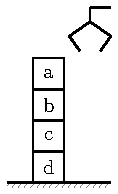
\includegraphics[width=0.5\textwidth,page=1]{examples/plan/block_world}
			\end{column}
		\end{columns}
		\par\bigskip
		Чему научишься:
		\begin{itemize}
			\item Познакомишься с тем, как программируют алгоритмы для искусственного интеллекта.
			\item Познакомишься с одним из самых известных алгоритмов планирования поведения.
			\item Узнаешь как писать код для ИИ на Python и как проводить с ним эксперименты.
		\end{itemize}
	\end{frame}

	\begin{frame}
		\frametitle{AI-Cognitive: Coalitions}
		
		\begin{columns}
			\begin{column}{0.5\textwidth}
				Для одной из систем моделирования многоагентных систем (Jadex - \url{activecomponents.org}) нужно разработать своего агента и провести с ним эксперименты.
			\end{column}
			\begin{column}{0.5\textwidth}
				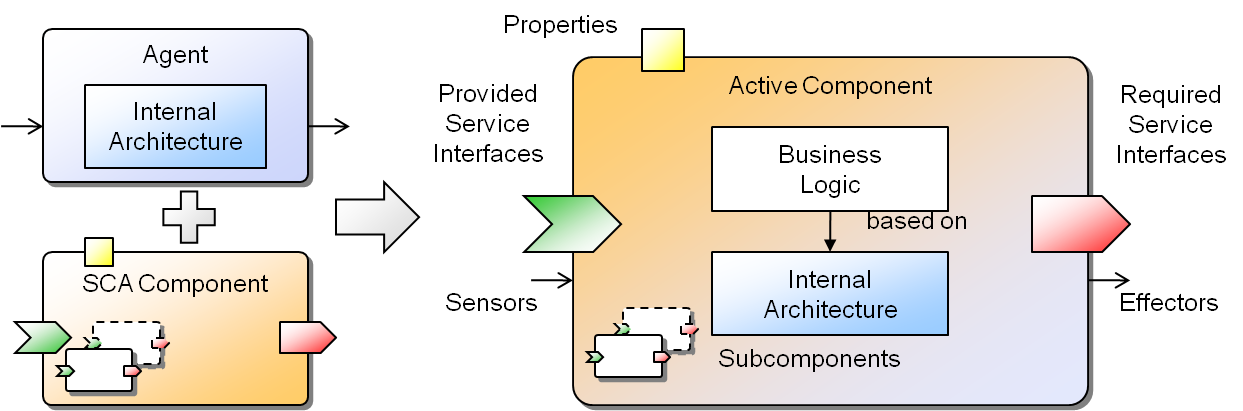
\includegraphics[width=\textwidth]{misc/agents/ac.png}
			\end{column}
		\end{columns}
		\par\bigskip
		Чему научишься:
		\begin{itemize}
			\item Познакомишься с современными системами искусственного интеллекта (ИИ).
			\item Разберешься с одной или несколькими задачками, где нужны усилия нескольких роботов (интеллектуальных агентов).
			\item Познакомишься с кодом, который реализует разные протоколы коммуникации.
		\end{itemize}
	\end{frame}

	\begin{frame}
		\frametitle{AI-Cognitive: Architectures}
		
		\begin{columns}
			\begin{column}{0.5\textwidth}
				C одной из архитектур управления (Soar - \url{soar.eecs.umich.edu} или ACT-R - \url{act-r.psy.cmu.edu}) предлагается познакомиться: поставить себе на компьютер дистрибутив системы, разобраться из каких модулей он состоит и как работает его ядро моделирования рассуждений.
			\end{column}
			\begin{column}{0.5\textwidth}
				\centering
				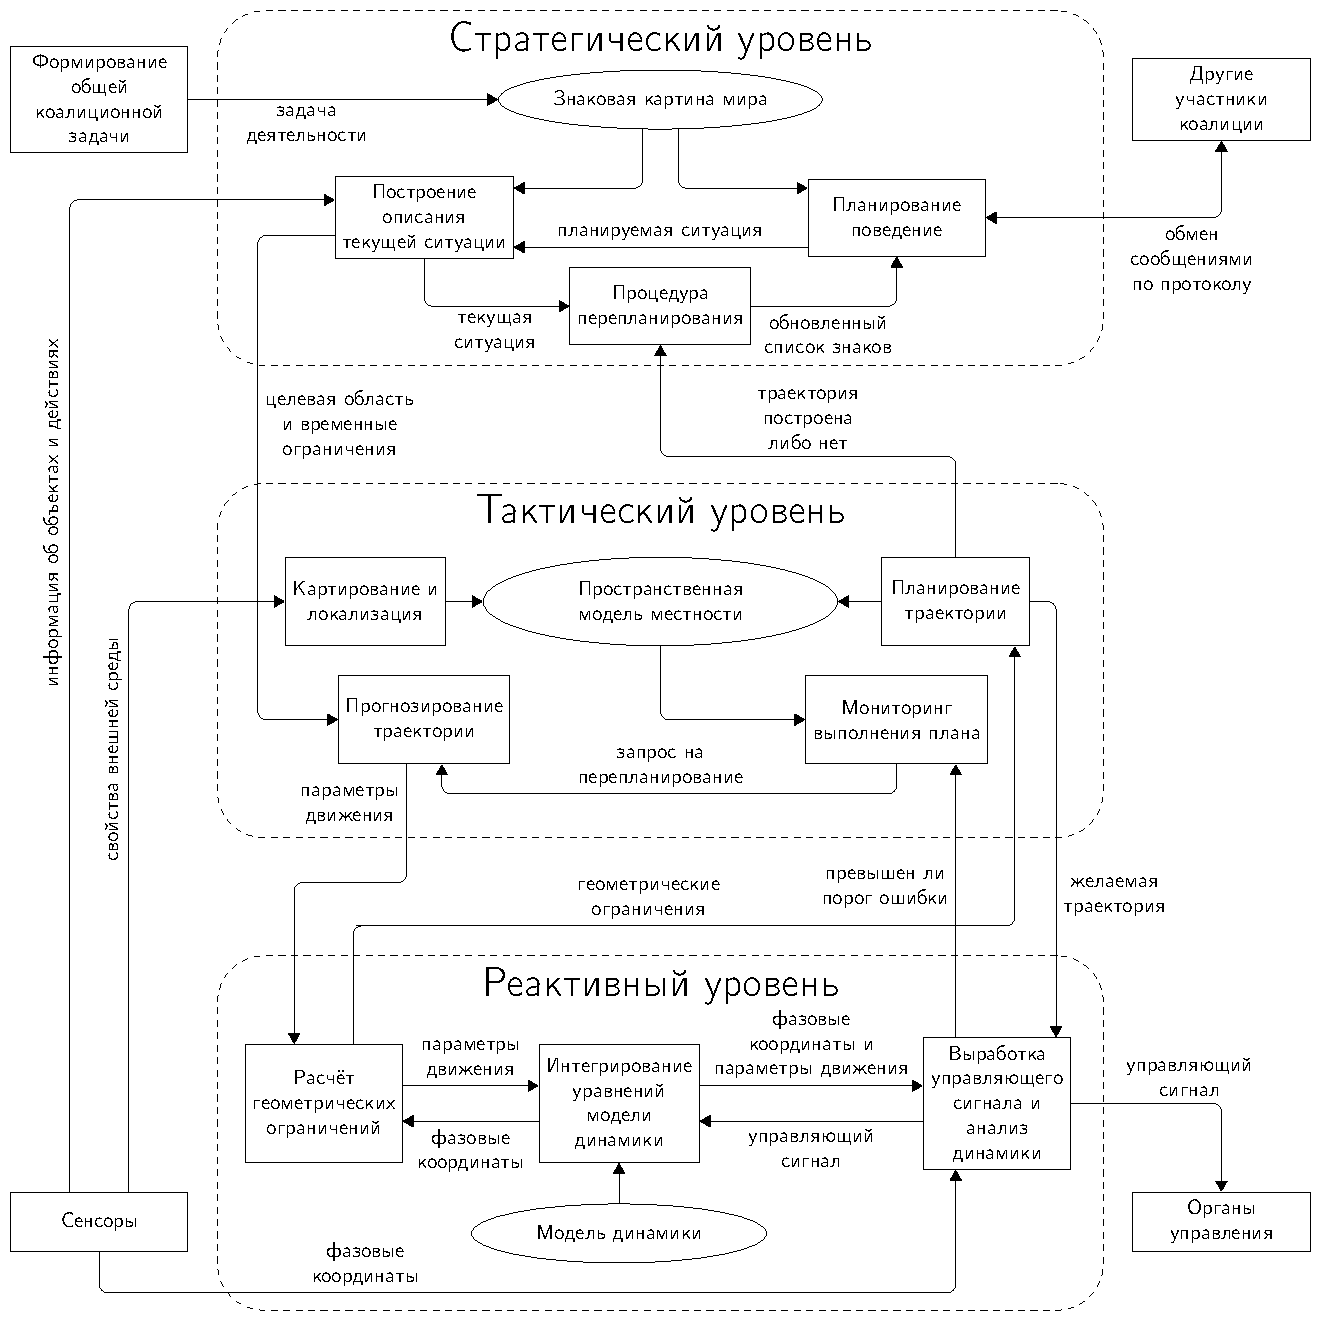
\includegraphics[width=0.8\textwidth]{agent-schemas/ru/architecture}
			\end{column}
		\end{columns}
		\par\bigskip
		Чему научишься:
		\begin{itemize}
			\item Познакомишься с современными система искусственного интеллекта.
			\item Разберешься с некоторыми важными алгоритмами ИИ.
			\item Узнаешь как ведется разработка систем управления ИИ.
		\end{itemize}
	\end{frame}
\end{document}
	
	
